\documentclass{article}

\usepackage[a4paper, margin=1in]{geometry}
\usepackage[onehalfspacing]{setspace} % Correct 1.5 line spacing

\usepackage{graphicx}  % Figures
\graphicspath{{../figures/}}

\usepackage{fontspec}  % Fonts
\usepackage{helvet}
\usepackage{newpxtext,newpxmath}
\defaultfontfeatures{Scale=MatchLowercase, Ligatures=TeX}

\usepackage{url}
\usepackage[pdfusetitle]{hyperref}
\usepackage{titlesec}      % Modify title/section/chapter commands
\usepackage{mathtools}     % Various maths related commands
\usepackage{gensymb}       % \degree symbol
\usepackage[thinc]{esdiff} % Derivatives
\usepackage{booktabs}      % \toprule, etc., in tables

% https://tex.stackexchange.com/a/43009
\DeclarePairedDelimiter\abs{\lvert}{\rvert}%
\DeclarePairedDelimiter\norm{\lVert}{\rVert}%

% Caption figures
\usepackage{caption}
\DeclareCaptionFont{captionlabelfont}{\bfseries \sffamily}
\DeclareCaptionFont{captiontextfont}{\sffamily}
\captionsetup{labelfont=captionlabelfont, textfont=captiontextfont}

% Change footnote style
\renewcommand{\thefootnote}{\fnsymbol{footnote}}

% Fancy header/footer
\usepackage{fancyhdr}
\pagestyle{fancy}
\renewcommand{\sectionmark}[1]{\markright{\thesection . #1}}
\fancyhf{}
\lhead{\fancyplain{}{\thepage}}
\rhead{\fancyplain{}{\textit{\rightmark}}}

% Bibliography
\usepackage[backend=biber, style=phys, natbib=true,
			url=false, isbn=false, doi=false, eprint=false,
			autocite=superscript]{biblatex}

\addbibresource{references.bib}

\newcommand\mytitle {Notes on FMCW and Meteorological Radar}
\newcommand\myauthor{Stuart Ballantyne}
\newcommand\mydate  {\today}

\title {\mytitle}
\author{\myauthor}
\date  {\mydate}

\begin{document}
	\maketitle
	\tableofcontents
	\newpage
	
	\begin{figure}
		\centering
		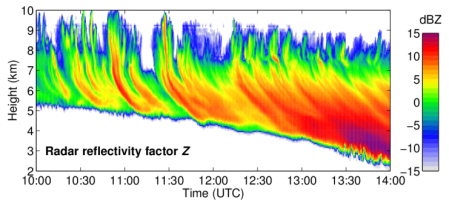
\includegraphics[width=0.8\textwidth]{example-output}
		\caption{Example cloud radar output.\supercite{ExampleOutput}}
		\label{fig:ExampleOutput}
	\end{figure}
	
	\section{Radar range equation}
	
	\subsection{Point target}
	Consider an isotropically emitting antenna with transmit power \(P_t\).
	The power density \(Q\) at a distance \(r\) from the antenna is given by
	\begin{equation*}
		Q = \frac{P_t}{4 \pi r^2}.
	\end{equation*}
	To account for the directivity and efficiency of the antenna one must include the (transmit) gain \(G_t\). Hence,
	\begin{equation*}
		Q = \frac{G_t P_t}{4 \pi r^2}.
	\end{equation*}
	The power reflected by a target with \textit{radar cross-section} \(\sigma\) (units of cross-sectional area) is then
	\begin{equation*}
		P_{refl} = Q \sigma = \frac{G_t P_t \sigma}{4\pi r^2}.
	\end{equation*}
	Assuming the power is reflected isotropically, then
	\begin{equation*}
		Q_r = \frac{P_{refl}}{4\pi r^2} = \frac{G_t P_t \sigma}{(4\pi r^2)^2}.
	\end{equation*}
	The receiver antenna has an effective area \(A\) given by
	\begin{equation*}
		A = \frac{G_r \lambda^2}{4\pi},
	\end{equation*}
	where \(G_r\) is the receiver antenna gain. The received power is simply the product \(P_r = A Q_r\), hence we finally arrive at
	\begin{equation}
		P_r = \frac{P_t G_t G_r \lambda^2}{(4\pi)^3 r^4} \sigma \label{eqn:PointRange},
	\end{equation}
	which is known as the \textbf{radar range equation}.
	
	\subsection{Meteorological targets}
	For a distributed meteorological target, one writes
	\begin{equation}
		\sigma = \eta V,
	\end{equation}
	where \(\eta\) is the volume reflectivity (cross-sectional area per unit volume) and \(V\) is the volume sampled by the radar.

	[Derive volume term]

	In the Rayleigh scattering regime, one can write
	\begin{equation}
		\eta = \sum_i{\sigma_i} = \frac{\pi^5}{\lambda^4} \abs{K}^2 \sum_i{D_i^6} = \frac{\pi^5}{\lambda^4} \abs{K}^2 Z
	\end{equation}
	
	Thus, the \textbf{meteorological radar range equation} is
	\begin{equation}
		P_r = \frac{P_t G_t G_r \lambda^2}{(4 \pi)^3 r^4} \cdot \frac{1}{2\ln{2}} \cdot \frac{\pi r^2 \theta \phi c \tau}{8} \cdot \eta = \frac{P_t G_t G_r \lambda^2 \theta \phi c \tau}{1024 (\ln{2}) \pi^2 r^2} \eta = \frac{P_t G_t G_r \theta \phi c \tau \pi^3 \abs{K}^2}{1024 (\ln{2}) \lambda^2 r^2} Z,
		\label{eqn:MeteoRange}
	\end{equation}
	where we have inserted a factor \(1/(2\ln{2})\) to account for the Gaussian antenna gain profile.\supercite{ProbertJones}

	\pagebreak

	\section{Frequency-modulated continuous wave}
	\begin{figure}
		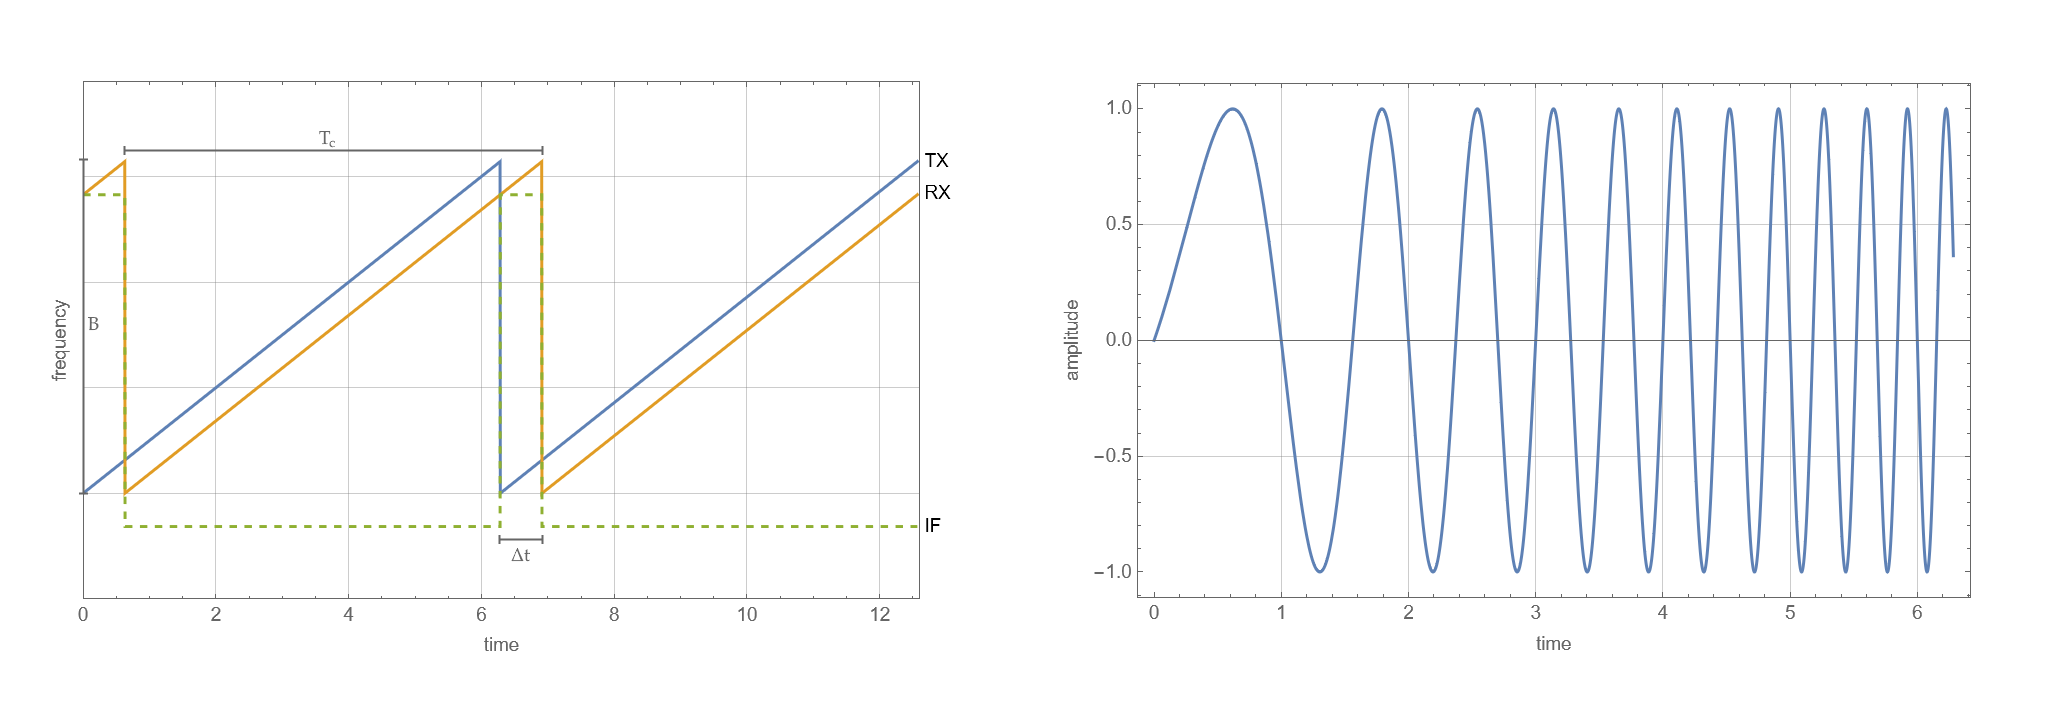
\includegraphics[width=\textwidth]{chirp-2}
		\caption{Left: transmitted (TX) and received (RX) sawtooth chirps and their difference frequency (IF). Right: illustration of TX chirp waveform (own work).}
		\label{fig:Chirp}
	\end{figure}

	\section{Radar reflectivity}
	\begin{table}
		\begin{minipage}[r]{0.3\textwidth}
			\begin{tabular}{|l|l|}
				\toprule
				Wavelength (mm)        & \(3.19\) \\
				Range res. (m)         & \(10\)   \\
				Transmit power (dBm)   & \(25\)   \\
				Gain (dBi)             & \(52\)   \\
				Beamwidth (\degree)    & \(0.43\) \\
				Chirp rep. freq. (GHz) & \(6510\) \\
				Noise figure (dB)      & \(5.3\)  \\
				\bottomrule
			\end{tabular}
		\caption{Parameters for the St. Andrews 94-GHz cloud profiling radar.\supercite{StAndrewsRadar}}
		\end{minipage}
	\end{table}

	\nocite{*} % Show all references.
	\printbibliography
\end{document}